\providecommand{\main}{../main}
\documentclass[\main/main.tex]{subfiles}
\graphicspath{{../images/}}
\begin{document}
\section{
    $ℤ₂$ゲージ理論
}
\begin{frame}{\currentname}
    ここからFradkinの内容。

    グラフ$G$を2次元正方格子とする。
    古典論では、各辺に2値を取る向きの自由度を考えた。
    これに対応する量子論の状態空間として、各辺$e$に対しスピン$1/2$のHilbert空間$ℋ_e$を考え、
    全ての辺についてテンソル積したもの考える。
    \begin{align}
        ℋ = ⨂_{e ∈ ℰ} ℋ_e,␣ ℋ_e ≅ \Span\{|0⟩,|1⟩\}
    \end{align}
    また$σ^z$の固有値$1$を右・上向きに、固有値$-1$を左・下向きに対応させる。
    ハミルトニアンを
    \begin{align}
        H = -g ∑_{e ∈ ℰ} σ^x(e)
            - ÷{1}{g}∑_{f ∈ ℱ} W(∂f)
            \label{eq: Hamiltonian of Z2 gauge theory}
    \end{align}
    と定義する。ここで$W(∂f)$はプラケット演算子
    \begin{align}
        W(∂f) ≔ ∏_{e ∈ ∂f} σ^z(e)
    \end{align}
    である。
\end{frame}
\begin{frame}{\currentname}
    頂点$α$に対し、バーテックス演算子を
    \begin{align}
        \~W(\~∂v) ≔ ∏_{e ∈ \~∂v} σ^x(e)
    \end{align}
    と定義する。
    この演算子は$\~W(\~∂v)² = 1$を満たし、
    コバウンダリー$\~∂v$に対する$ℤ₂$ゲージ変換を生成する。
    ゲージ不変な状態は
    \begin{align}
        \~W(\~∂v)|\Phys⟩ = |\Phys⟩
    \end{align}
    を満たす。
    容易に
    \begin{align}
        [\~W(\~∂v),\~W(\~∂v')] = 0,␣ [\~W(\~∂v'),H] = 0
    \end{align}
    が示せるので、$\{\~W(\~∂v)\},H$を同時対角化できる。
    よって任意のゲージ変換について不変な状態をとってこれる。
\end{frame}
\begin{frame}{\currentname}
    ゲージ不変な物理量は以下の通り。 3.はゲージ不変なのか?
    \begin{enumerate}
        \item サイクル$Γ$上のWilsonループ
        \begin{align}
            W(Γ) = ∏_{e ∈ Γ}σ^z(e)
        \end{align}
        \item 辺$e$上の電場 $σ^x(e)$
        \item 頂点$v$上の電荷。
        \begin{align}
            W(γ_{v,∞}) = ∏_{e ∈ γ_{v,∞}} σ^z(e)
        \end{align}
        ただし$γ_{v,∞}$は$v$と無限遠点を端点にもつチェイン。
        \item 非自明なコサイクル$\~Γ$上の 't Hooft ループ
        \begin{align}
            \~W(\~Γ) = ∏_{e ∈ \~Γ} σ^x(e)
        \end{align}
        \item 面$f$上の磁荷
        \begin{align}
            τ^z(f) = \~W(\~γ_{v,∞})
            = ∏_{e ∈ \~γ_{f,∞}} σ^x(e)
        \end{align}
        ただし$\~γ_{f,∞}$は$f$と無限遠点を端点にもつコチェイン。
    \end{enumerate}
\end{frame}
\begin{frame}{\currentname}
    ハミルトニアン(\ref{eq: Hamiltonian of Z2 gauge theory})
    を双対格子の言葉に直そう。
    磁荷演算子$τ^z(f)$はWilsonループ$W(∂f)$と反交換する。
    \begin{align}
        {W(∂f),τ^z(f)} = 0
    \end{align}
    $W(∂f)² = 1$から、
    Wilsonループは双対格子上のPauli行列$τ^x(f) ≔ W(∂f)$とみなすことができる。
    また
    \begin{align}
        σ^x(e) = ∏_{f ∈ \~∂e}τ^z(f)
    \end{align}
    が成り立つ。よって、
    \begin{align}
        H = -g∑_{⟨f,f'⟩}τ^z(f)τ^z(f') - ÷{1}{g}∑_f τ^x(f)
    \end{align}
    となる。なんと、横磁場Ising模型になった。
    ということで、横磁場Ising模型は$(2+1)$次元$ℤ₂$ゲージ理論と双対の関係にある。
    $τ^z$は横磁場Ising模型の秩序変数だが、ゲージ理論側では磁荷に対応する。
\end{frame}
\section{
    $ℤ₂$閉じ込め相
}
\begin{frame}{\currentname}
    $g$が大きい場合には強結合展開(低温展開)を行える。
    $-g∑_e σ^x(e)$が支配的なので基底状態は
    \begin{align}
        |𝐺_∞⟩ = ∏_{e ∈ ℰ}|σ^x(e) = +1⟩
    \end{align}
    となる。

    励起状態を作るためには$σ^x$をフリップすればよいが、
    ゲージ不変性から$σ^x = -1$の辺はサイクルをなす必要がある。
    つまり真空にWilsonループを作用させることで励起状態を構成できる。
    $W(Γ)|𝐺_∞⟩$の励起エネルギーは、
    \begin{align}
        𝛥E = 2g|Γ|
    \end{align}
    で与えられる。

    $g$が有限の場合、基底状態はループ状の励起の重ね合わせで表される。
    $g → g_𝑐$とすると、ギャップは0に近づき、
    典型的なループの大きさが発散するため、
    強結合展開は破綻する。

    双対な横磁場Ising模型では、
    $g → ∞$はIsing相互作用が横磁場に比べて大きい極限なので、秩序相に対応する。
    これはモノポール$τ^z(f)$が凝縮した相とみなすことができる。
\end{frame}
\begin{frame}{\currentname}
    単一電荷が存在する状態は、
    \begin{align}
        Q(v₀)|ψ⟩ = -|ψ⟩,␣ Q(v)|ψ⟩ = |ψ⟩␣(v ≠ v₀)
    \end{align}
    で定義される。基底状態からこの状態を作ろうとすると、
    \begin{align}
        |ψ⟩ = W(γ_{v₀,∞})|𝐺⟩
        = ∏_{e ∈ γ_{v₀,∞}}σ^z(e) |𝐺⟩
    \end{align}
    とする必要がある。ここで$γ_{v₀,∞}$は$v₀$と無限遠点を端点にもつチェインである。
    このためには無限の$σ^x$をフリップしないといけないので、
    gappedな相では単一の電荷を作ることはできない。

    ただし、基底状態にWilsonラインを作用させることで、
    2つの電荷の対ならば有限のエネルギーで作ることができる。
    $R$だけ離れた電荷の間のエネルギーは
    \begin{align}
        𝛥E(R)  = σR,␣ σ = 2g + O(1/g)
    \end{align}
    となる。$σ$を "string tension" と呼ぶ。$σ$は$g → g_𝑐$で0に近づく。

    これは$\SU(3)$ゲージ理論の強結合領域で電荷(色荷)が単独で存在できない事情と同じなので、
    これをもって$ℤ₂$閉じ込め相と呼ぶ。
\end{frame}
\begin{frame}{\currentname}
    次にWilsonループの期待値を考える。
    まず$g = ∞$では$⟨𝐺_∞|W(∂S)|𝐺_∞⟩ = 0$である。
    有限の$g$では$|𝐺⟩$はBrillouin-Wigner摂動論によって$1/g²$で展開できる。
    有限の寄与が出てくるのは$|S|$は面$S$の面積として、$(1/g²)^{|S|}$次以降であるから
    \begin{align}
        ⟨𝐺(g)|W(∂S)|𝐺(g)⟩ ∼ (÷{1}{g²})^{|S|}
        = ℯ^{-μ(g)|S|},␣
        μ(g) = \log(g²) + 𝒪(1)
    \end{align}
    となるだろう。
    
    かなり雑に議論してしまったので、ちゃんと考えてみる。
    まず
    \begin{align}
        H = g(E_∞ + H_∞ - ÷{1}{g²} ∑_f W(∂f)),␣
        H_∞ = ∑_{e ∈ ℰ}(1-σ^x(e))
    \end{align}
    とおく。ここで$gE_∞$は$g = ∞$での基底状態のエネルギーを表す。
    基底状態$|𝐺⟩$は以下の自己無撞着方程式を満たす。
    \begin{align}
        |𝐺⟩ = |𝐺_∞⟩ + ÷{1}{g²}
         ÷{1-|𝐺_∞⟩⟨𝐺_∞|}{H_∞ + ÷{1}{g²} ∑_f ⟨𝐺_∞|W(∂f)|𝐺⟩}
         ∑_f W(∂f)|𝐺⟩
     \end{align}
     である。
\end{frame}
\begin{frame}{\currentname}
    $g → ∞$で主要な項を取り出すと、
    \begin{align}
       ⟨𝐺|W(∂S)|𝐺⟩
       ≈ (÷{1}{g²})^{|S|}∑⟨𝐺|W(∂S)∏_{f_i ∈ S}÷{W(∂f_i)}{H_∞}|𝐺_∞⟩
    \end{align}
    と書ける。
    $∑$はWilsonループを掛けるあらゆる順序についての足し合わせである。
    これを平均場近似を使って評価しよう。
    $S$の中でランダムに面を塗りつぶして行って、$S' ⊂ S$を構成する。
    このとき$∂S'$の長さは
    \begin{align}
        |∂S'| ≈ 2|S|⋅2p(1-p),␣ p = ÷{|S'|}{|S|}
    \end{align}
    と評価できる。
    ここで$S$の内部に含まれる辺の総数がおおよそ$2|S|$であることを用いた。
    ここから
    \begin{align}
        ÷{1}{H_∞}∏_{f_i∈S'⊂S}W(∂f_i)|𝐺_∞⟩
        &
        ≈ ÷{1}{2|∂S'|}∏_{f_i∈S'⊂S}W(∂f_i)|𝐺_∞⟩\∅
        &
        = ÷{|S|}{8|S'|(|S|-|S'|)}
            ∏_{f_i∈S'⊂S}W(∂f_i)|𝐺_∞⟩
    \end{align}
    となる。
\end{frame}
\begin{frame}{\currentname}
    よって
    \begin{align}
        ⟨𝐺|W(∂S)|𝐺⟩
        &
        ≈ (÷{1}{g²})^{|S|}(|S|+1)! ∏_{n = 1}^{|S|}
            ÷{|S|}{8n(|S|-n)}\∅
            &
        = (÷{|S|}{8g²})^{|S|}÷{(|S|+1)!}{(|S|!)²}\∅
        &
        ∼  \exp(\log(|S|/8g²)|S| - |S|\log |S| + |S|)\∅
        &
        = \exp(-μ(g)|S|)
    \end{align}
    となる。
    ここで、$μ(g) = \log(8g²) - 1$である。
    \footnote{
        相転移点を$μ(g)=0$となる点とすれば、$1/g_𝑐² ∼ 8/ℯ = 2.94$と推定できる。
        これを数値計算の結果$1/g_𝑐² = 3.044$と比較すると、割といい線いっている。
    }

    粗っぽい評価だが、Wilsonループの期待値が閉じ込め相で面積則に従うことがわかった!

    疑問: 面積則は閉じ込め相に対して普遍的な性質か?
\end{frame}
\section{
    $ℤ₂$非閉じ込め相
}
\begin{frame}{\currentname}
    次に弱結合相を考える。
    $g → 0$の基底状態は全てのプラケット演算子$W(∂f)$に対して
    固有値$1$をもつ状態である。
    これは$ℤ₂$ゲージ場が平坦であると言い換えることができる。
    $W(∂f)$に対して対角化された基底は
    \begin{align}
        |{A}⟩ = ⨂_e |σ^z(e) = (-1)^{A(e)}⟩
    \end{align}
    のように書ける。$W(∂f)$について固有値が$1$となるのは
    \begin{align}
        W(∂f)|{A}⟩ = (-1)^{\~∂A(f)}|{A}⟩ = |{A}⟩
    \end{align}
    となるとき。すなわち$A$がコサイクル(閉形式)であるとき。

    ゲージ変換で移り合う状態を同一視するとき、ゲージ固定をすると便利である。
    \footnote{
        古典ダイマー模型におけるFisher-Kasteleyn-Temperleyのアルゴリズムとは、まさにゲージ固定を系統的に構成する方法である。
    }
    ここでは正方格子において$x$軸方向の辺で全て$σ^z = 1$とするゲージをとる。
    このとき基底状態は
    \begin{align}
        |𝐺₀⟩ = ⨂_{e ∈ ℰ}|σ^z(e) = 1⟩
    \end{align}
    となる。
\end{frame}

\begin{frame}{\currentname}
    ゲージ変換で移り合う基底を手で同一視するのではなく、
    そもそもゲージ不変な基底状態を構成することも可能である。
    この場合、
    $W(∂f)$だけでなく$\~W(\~∂v)$についても対角化するので、
    Toric code
    \begin{align}
        H = - ∑_f W(∂f) - ∑_{v ∈ 𝒱}\~W(\~∂v)
    \end{align}
    の基底状態を求めれば良い。(別に今はToricとは限定していないが。)
    これはKitaev状態
    \begin{align}
        |𝐺⟩_\𝚞{Kitaev} = ∑_{A ∼ A₀}|{A}⟩
    \end{align}
    として与えられる。
    ここで$A ∼ A₀$は$A = A₀ + \~∂Λ$を意味する。
    $|{A}⟩$は $A = ∑_e A(e)e$ に対して
    \begin{align}
        |{A}⟩ = ⨂_e |σ^z(e) = (-1)^{A(e)}⟩
    \end{align}
    として定義される。
    ゲージ変換はコホモロジー類の元に対する置換として作用するので、
    同じ重みで重ね合わせた$|𝐺⟩_\𝚞{Kitaev}$は任意のゲージ変換について不変になっている。
\end{frame}

\begin{frame}{\currentname}
    励起状態について考えよう。

    $|𝐺⟩_\𝚞{Kitaev}$に 't Hooft ライン$\~W(\~γ) = ∏_{e ∈ \~γ}σ^x(e)$を掛ければ、
    モノポール$τ^z(f)$の対を生成できる。
    $g=0$では励起エネルギーは常にモノポールと重なる$W(∂f)$に対して発生し、
    モノポール間の距離は関係ない。
    つまりモノポール間のポテンシャルは$0$である。

    次に$|𝐺⟩_\𝚞{Kitaev}$に Wilson ライン
    $W(γ) = ∏_{e ∈ γ}σ^z(e)$を掛ければ、
    電荷の対を生成できる。
    $g=0$では電荷はゲージ対称性を破るだけで、エネルギーは$0$である。
    $g > 0$では基底状態に$g²$のオーダーの寄与が加わるため、
    $R$だけ離れた電荷の間のエネルギーは
    \begin{align}
        𝛥E(R) = 2E₀(g) + V(g,R)
    \end{align}
    と書ける。ただし
    \begin{align}
        E₀(g) ∝ g² + O(g⁴),␣
        V(g,R) ∼ A(g)ℯ^{-R/ξ_s(g)}
    \end{align}
    である。
    gappedな相なので$V(g,R)$の$R$依存性が指数関数になるとした。

    これは電荷が遮蔽されていると捉えることもできる。
    電荷の対を生成して無限遠まで離していく過程で有限のエネルギーしか必要でないので、
    弱結合相を非閉じ込め相と呼ぶ。
\end{frame}
\begin{frame}{\currentname}
    Wilsonループの期待値は$g=0$においては
    \begin{align}
        ⟨𝐺₀|W(∂S)|𝐺₀⟩ = 1
    \end{align}
    である。
    $g > 0$では基底状態は束縛されたモノポール対が希薄気体と考えられる。
    Wilsonループの期待値はWilsonループがモノポール対と交差するごとに$-1$倍される。よってモノポール対の密度を$ρ(g)$とすると
    \begin{align}
        ⟨G|W(∂S)|G⟩ ≈ (1-ρ(g))^{|∂S|} ≈ ℯ^{-ρ(g)|∂S|}
    \end{align}
    と考えられ、Wilsonループの期待値が周長則に従うことがわかる。

    これもちゃんと考えたいなら摂動論を使うのがいいだろう。
    基底状態は
    \begin{align}
        |𝐺⟩ = |𝐺₀⟩ + g²÷{1-|𝐺₀⟩⟨𝐺₀|}{H₀+g²∑_e ⟨𝐺₀|σ^x(e)|𝐺⟩} ∑_e σ^x(e)|𝐺⟩
    \end{align}
    満たす。
\end{frame}
\begin{frame}{\currentname}
    モノポール対が$n$個ある状態を$|n⟩$と書くと、
    モノポール対が希薄であるとき
    \begin{align}
        ÷{1}{H₀+g²∑_e ⟨𝐺₀|σ^x(e)|𝐺⟩}|n⟩
        ≈ ÷{1}{H₀}|n⟩ ≈ ÷{1}{2n}|n⟩
    \end{align}
    としてしまってよい。よって
    \begin{align}
        |𝐺⟩
        &
        ≈ |𝐺₀⟩ + ÷{g²}{2} ∑_e σ^x(e)|𝐺₀⟩
        + ÷{1}{2!} (÷{g²}{2})² ∑_{e,e'}σ^x(e)σ^x(e')
            |𝐺₀⟩
        + ⋯ \∅
        &
        = ∏_e \exp(÷{g²}{2}σ^x(e))|𝐺₀⟩
    \end{align}
    となり、
    \begin{align}
        ⟨𝐺|W(∂S)|𝐺⟩ ≈ ∏_{e ∉ ∂S}\cosh(g²) ∏_{e ∈ ∂S} 1
    \end{align}
    と計算できる。
    ただし、これは発散するので以下のように規格化して、周長則を得る。
    \begin{align}
        ÷{⟨𝐺|W(∂S)|𝐺⟩}{⟨𝐺|𝐺⟩} ≈ ∏_{e ∈ ∂S}÷{1}{\cosh(g²)} = ℯ^{-\log(\cosh(g²))|∂S|}
    \end{align}
\end{frame}

\section{
    境界条件とトポロジー
}
\begin{frame}{\currentname}
    境界条件の影響を考えよう。

    閉じ込め相を双対な模型で考えると、
    基底状態では$τ^z(f)τ^z(f') = 1$が任意の辺$⟨f,f'⟩$について成り立つ。
    しかし、このような状態は$τ^z(f)$が全て$1$か全て$-1$かの2通りある。
    したがって双対変換は2対1の対応になっており、
    一方での対称性の破れが他方で区別されない。

    このような微妙な状況は、
    $ℤ₂$グローバル対称性変換を生成する演算子を考えてみると浮き彫りになる。
    これは
    \begin{align}
        \~Q = ∏_f τ^x(f)
        = ∏_{e ∈ ∑_f ∂f} σ^z(e) = W(∂M)
    \end{align}
    と表される。
    ここで$∂M = ∑_f ∂f$はグラフ全体の境界である。
    境界があるグラフでは、
    $⟨𝐺_∞|\~Q|𝐺_∞⟩ = 0$
    となる。
    一方$∂M = 0$ならば$W(∂M)=1$となり、Hilbert空間は$ℤ₂$対称なセクターに限られる。
\end{frame}
\begin{frame}{\currentname}
    次に、非閉じ込め相を考えてみよう。
    平坦な$ℤ₂$ゲージ場$A$に対するコホモロジー類は$2^{2g}$個存在する。
    ここでの$g$は種数なので注意。
    異なるコホモロジー類への変換はラージゲージ変換として、
    \begin{align}
        A → A + \~Γ_i␣ (\~∂\~Γ_i = 0,~ \~Γ_i ≁ 0)
    \end{align}
    で与えられる。

    トーラスの場合、ホモロジー類とコホモロジー類の代表元として
    $Γ₁,Γ₂,\~Γ₁,\~Γ₂$を取ってこれる。
    これらはそれぞれ$x$方向と$y$方向にのびるサイクル・コサイクルであり、
    \begin{align}
        (\~Γ₁,Γ₁) = 0,␣
        (\~Γ₁,Γ₂) = 1,␣
        (\~Γ₂,Γ₁) = 1,␣
        (\~Γ₂,Γ₂) = 0
    \end{align}
    が成り立つ。
    量子論でラージゲージ変換を生成するのは可縮でない 't Hooft ループ
    \begin{align}
        \~W(\~Γ_i) = ∏_{e ∈ \~Γ_i} σ^x(e)
    \end{align}
    である。
    Wilson ループと 't Hooft ループの間には
    \begin{align}
        W(Γ_i)\~W(\~Γ_j) = (-1)^{(Γ_i,\~Γ_j)} \~W(\~Γ_j)W(Γ_i)
    \end{align}
    という関係が成り立つ。
\end{frame}
\begin{frame}{\currentname}
    基底状態はコホモロジー類の数に対応して4重縮退している。
    これらは$\~W(\~Γ₁),\~W(\~Γ₂)$ (または$W(Γ₁),W(Γ₂)$) の固有値によって識別される。

    さらに、この縮退は$g = 0$だけの特殊事情ではない。
    $|𝐺₀⟩$に 't Hooftラインや可縮なWilsonループを作用させても$\~W(\~Γ_i)$の固有値を変えることはない。
    可縮でないWilsonループは$\~W(\~Γ_i)$の固有値を変えるが、
    この励起はエネルギーが大きすぎるため無視できる。
    よってトポロジカルな縮退は有限の$g$まで維持される。

    以上のような縮退は自発的対称性の破れとはメカニズムが全く異なるものである。
    境界条件によって縮退度が変化するという特徴をもつ相はトポロジカル相と呼ばれる。
    非閉じ込め相にある$ℤ₂$ゲージ理論は$ℤ₂$トポロジカル流体の例である。
    また量子Hall系もトポロジカル相であり、後の章で扱われる。
\end{frame}
\section{
    物質場を入れた$ℤ₂$ゲージ理論
}
\begin{frame}{\currentname}
    物質場として$ℤ₂$係数$0$-形式場$τ(v)$を考える。
    ゲージ場$A(e)$と物質場$τ(v)$に対するゲージ変換は
    \begin{align}
        A(e) → A(e) +\~∂Λ(e),␣
        τ(v) → (-1)^{Λ(v)} τ(v)
    \end{align}
    と定義される。物質場に対応するHilbert空間として
    \begin{align}
        τ(v) = ±1 → |τ^z(v) = ±1⟩
    \end{align}
    を考える。するとゲージ変換は演算子
    \begin{align}
        Q(v) ≔ \~W(\~∂v)τ^x(v)
        = (∏_{e ∈ \~∂v}σ^x(e))τ^x(v)
    \end{align}
    として表される。そこで、ハミルトニアンを
    \begin{align}
        H =&- g ∑_e σ^x(e)
            - ÷{1}{g} ∑_f W(∂f)\∅
            &
            - ÷{1}{λ} ∑_v τ^x(v)
            - λ ∑_{⟨v,v'⟩} τ^z(v)σ^z(⟨v,v'⟩)τ^z(v')
    \end{align}
    とする。各項が$Q(v)$と可換なことに注意。
\end{frame}
\begin{frame}{\currentname}
    $v,v'$を端点にもつチェイン$γ_{v,v'}$に対し、
    以下の演算子を考える。
    \begin{align}
        C(γ_{v,v'})
        = τ^z(v)(∏_{e ∈ γ_{v,v'}}σ^z(e))τ^z(v')
    \end{align}
    これは電荷の対を作り出す演算子だが、
    先程と異なりゲージ変換と可換である。
    $v,v'$を引き離していくと、孤立した電荷が得られる。

    孤立した電荷はペアの電荷を無限遠に追いやって忘れることではじめて現れる概念である。
    このような機構をFradkinは"fractionalization"と呼んでいる。
    例えば整数電荷の集まりであるはずの2次元電子系で分数電荷が現れるのも同じようなからくりである。
\end{frame}
\begin{frame}{\currentname}
    ユニタリーゲージ
    \begin{align}
        τ^z(v)|\Phys⟩ = |\Phys⟩
    \end{align}
    をとる。
    このとき物質場の自由度を除いたハミルトニアンは
    \begin{align}
        H =&- g ∑_e σ^x(e)
            - ÷{1}{g} ∑_f W(∂f)\∅
            &
            - ÷{1}{λ} ∑_v \~W(\~∂v)
            - λ ∑_e σ^z(e)
    \end{align}
    と表される。
    このハミルトニアンにおいて格子を双対変換し、$σ^x ↔ σ^z$と取り替えると、
    結合定数を
    \begin{align}
        λ ↔ g
    \end{align}
    としたハミルトニアンが得られる。
    これらのハミルトニアンは双対の関係にある。
\end{frame}
\begin{frame}{\currentname}
    相図は以下のようになる。
    実線は連続相転移で、破線は2次相転移を表す。
    \begin{figure}[H]
        \centering
        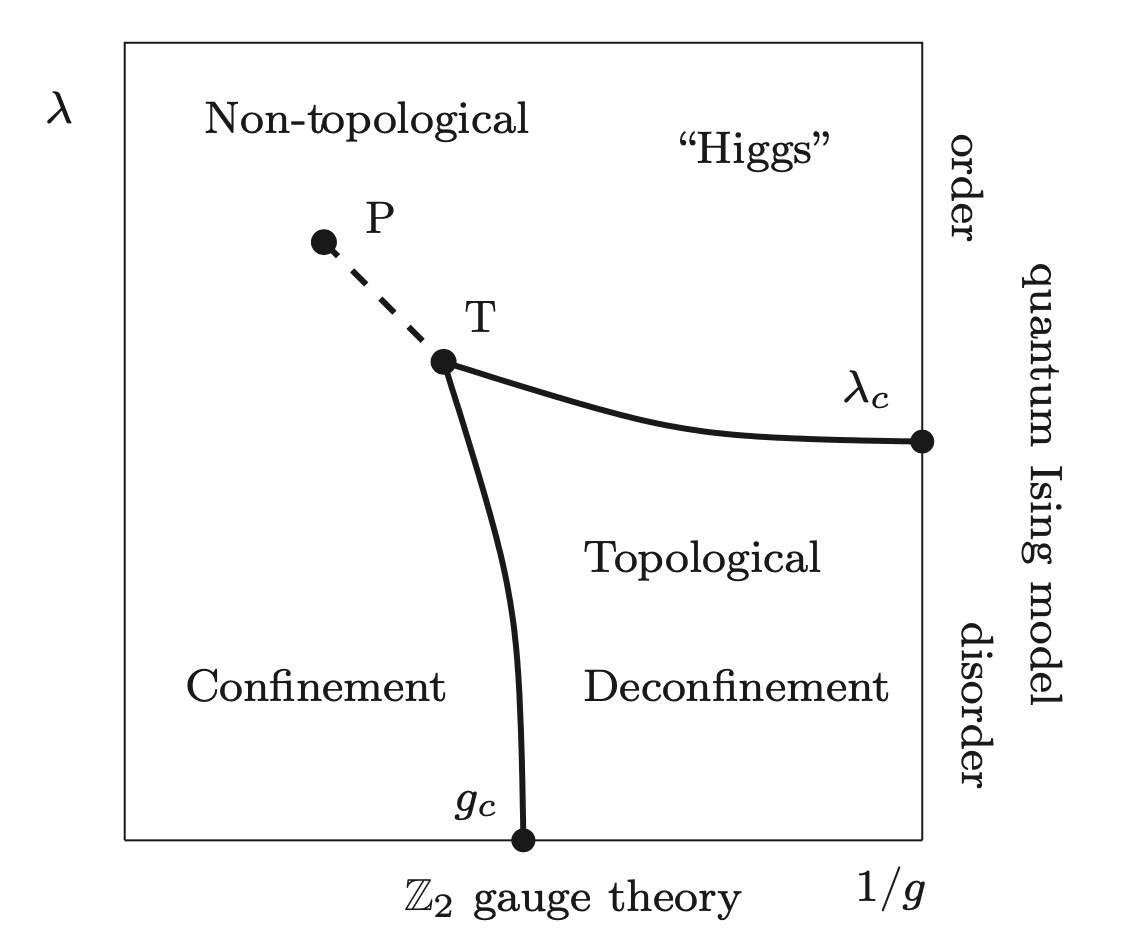
\includegraphics[width=0.7\hsize]{Z2gaugematter.png}
    \end{figure}
\end{frame}
\section{
    CQED
}
\begin{frame}{\currentname}
    格子上の$U(1)$ゲージ理論において、
    以下のようなハミルトニアンを考える。
    \begin{align}
        H_\𝚞{CQED}
        = ÷{g}{2}∑_e E(e)² 
        - ÷{1}{g} ∑_f\cos F(f)
    \end{align}
    ただし$F = \~∂A$である。
    ハミルトニアンの各項はゲージ変換を生成する演算子
    $Q(v) = ∂E(v)$と交換する。
    ゲージ不変なセクターは
    \begin{align}
        Q(v)|\Phys⟩ = 0
    \end{align}
    によって定義される。

    CQEDはQDMと似ているが、
    \begin{enumerate}
        \item[(a)] 共鳴項$ ∑_f \cos F(f)$の符号が異なる。
        \item[(b)] 拘束条件$∂E = ρ$において、QDMではstaggerdな背景電荷がある。
    \end{enumerate}
    (a)に関しては$A → A + a,~\~∂a = 𝜋$とすればすぐに解消できる。
    一方(b)は変数の取り替えによって除くことはできない。
\end{frame}
\begin{frame}{\currentname}
    $(2+1)$次元ではCQEDは$g > 0$で閉じ込め相にあることが知られている。
    $g = ∞$での基底状態は$|{E(e) = 0}⟩$である。
    Wilsonライン
    \begin{align}
        W(γ_{x,y}) = ∏_{e ∈ γ_{x,y}}ℯ^{¡qA(e)}
    \end{align}
    によって、電荷の対を生成できる。
    実際、
    \begin{align}&
        W(γ_{x,y})Q(x)
        = (Q(x)+q)W(γ_{x,y}),\\
        &
        W(γ_{x,y})Q(y)
        = (Q(y)-q)W(γ_{x,y})
    \end{align}
    となる。
    このとき
    \begin{align}
        𝛥E(|x-y|) = ÷{gq²}{2}|x-y|
    \end{align}
    であるから、電荷が孤立して存在するためには無限のエネルギーが必要であり、
    閉じ込めが起こる。

    $g = +0$まで閉じ込め相が続くのは非自明であるが、後で議論する双対変換によって理解できる。
\end{frame}
\section{
    $\U(1)$ゲージ理論におけるトポロジカル相
}
\begin{frame}{\currentname}
    物質場として角度変数${θ(v)}$を考え、
    共役運動量を${L(v)}$とする。
    \begin{align}
        [θ(v),L(v')] = ¡δ_{v,v'}
    \end{align}
    物質場の電荷を$q$とする。
    ゲージ変換は
    \begin{align}
        A(e) → A(e) + \~∂α(e),␣
        θ(v) → θ(v) + qα(v)
    \end{align}
    と定義される。この変換の生成子は
    \begin{align}
        Q(v) = ∂E(v) + qL(v)
    \end{align}
    である。ゲージ不変な状態は$Q(v)|\Phys⟩ = 0$を満たす。
\end{frame}
\begin{frame}{\currentname}
    ハミルトニアンを
    \begin{align}
        H =&∑_v ÷{1}{2λ} L(v)²
            - ∑_e λ\cos(\~∂θ(e)-qA(e))\∅
            &
            + ÷{g}{2} ∑_e E(e)²
            - ÷{1}{g} ∑_f \cos(\~∂A(f))
    \end{align}
    とする。
    第1項は角度変数のダイナミカルな項であり、
    第2項は共変微分による運動項
    \begin{align}
        Dℯ^{-¡θ}∧★Dℯ^{¡θ}
        = (\𝑑{θ}-qA)∧★(\𝑑{θ}-qA)
    \end{align}
    の離散的な対応物である。
    また$θ ∈ ℝ/2𝜋ℤ$からcosの中に入れる必要がある。
\end{frame}
\begin{frame}{\currentname}
    相図は以下のようになる。
    実線が1次相転移で、破線が連続相転移である。
    各領域について、これから説明する。
    \begin{figure}[H]
        \centering
        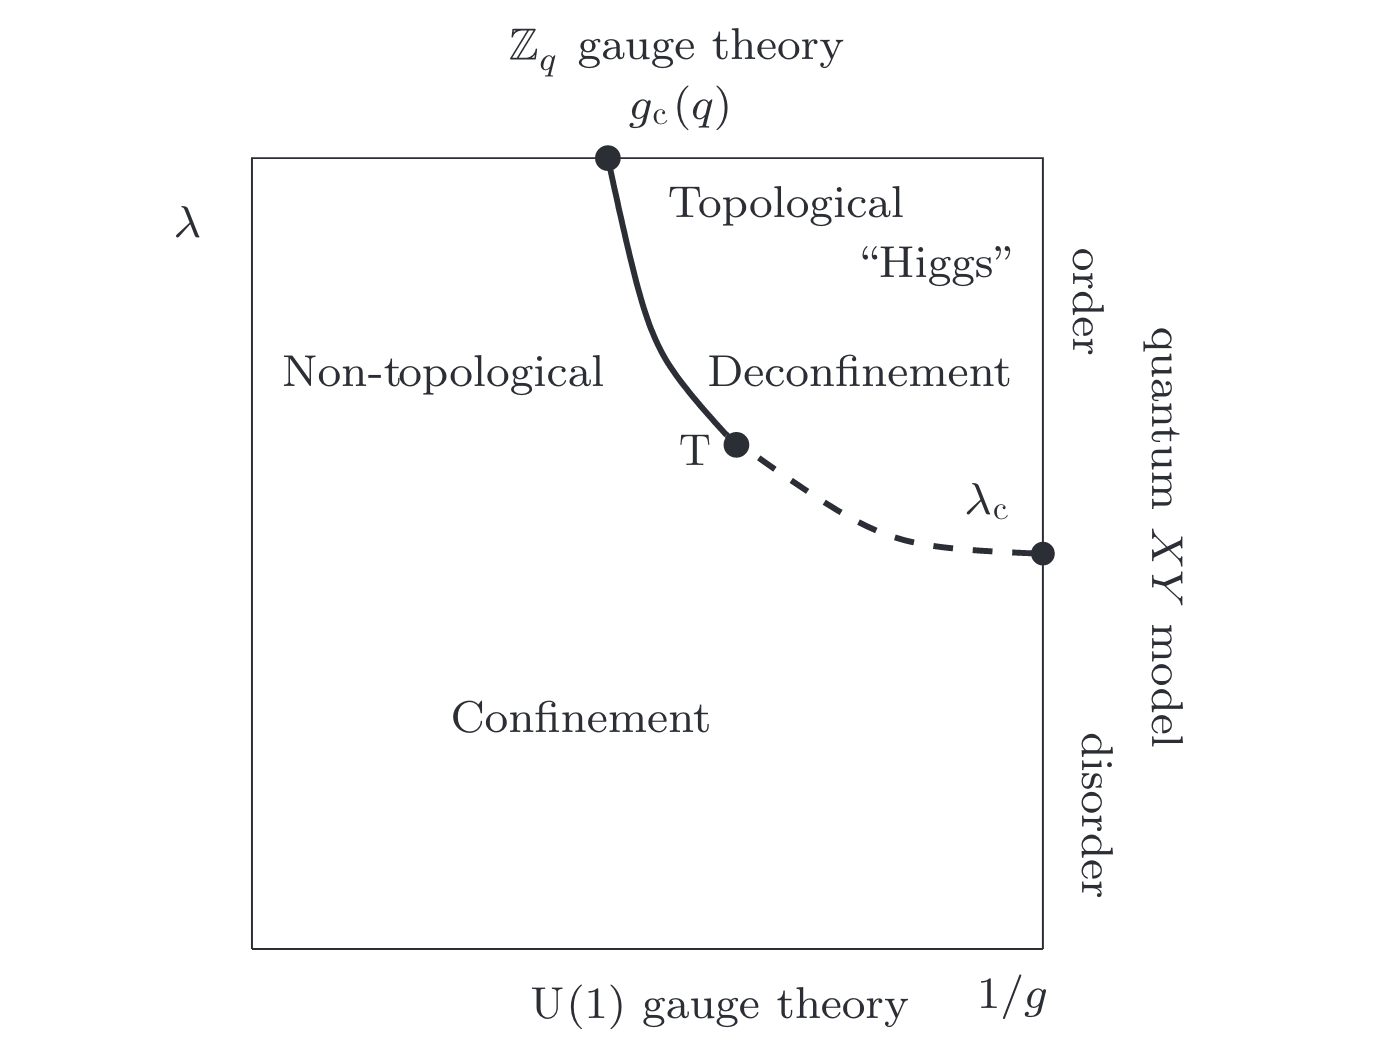
\includegraphics[width=0.7\hsize]{U1gauge.png}
    \end{figure}
\end{frame}
\begin{frame}{\currentname}
    $λ = 0$の場合、$L(v) = 0$となる。
    ゲージ不変性からこれは$∂E(v) = 0$を意味し、電荷の自己エネルギーが発散する。
    よって閉じ込め相が実現する。
    
    $g = ∞$の場合、$E(e) = 0$となる。
    このときWilsonラインによる励起エネルギーがその長さに比例するので、
    閉じ込め相が実現する。

    $g = 0$の場合は$A$が平坦になり、ゲージ変換によって局所的には$A = 0$とおくことができる。
    $A $に対してラージゲージ変換を行うことは、$θ$に対してトポロジカル欠陥を作ることに対応する。
    このようにして$A$を取り除くとグローバル$\U(1)$対称性をもつ quantum-rotor model が得られる。

    quantum-rotor modelにおいて、
    $λ < λ_𝑐$であればおおよそ$L(v) = 0$となり、
    基底状態はグローバル$\U(1)$対称性をもつ。
    $λ < λ_𝑐$では自発的に対称性が破れ、gaplessな南部-Goldstoneモードが現れる。
    $g ≠ 0$の場合はゲージ場が南部-Goldstoneモードと結合することでHigssモードになる。
\end{frame}
\begin{frame}{\currentname}
    $λ → ∞$では$ℤ_q$ゲージ理論が現れる。
    ユニタリーゲージ$θ = 0$をとれば、$A(e)$が取りうる値は
    \begin{align}
        A(e) = ÷{2𝜋}{q}p(e),␣ p(e) ∈ ℤ_q
    \end{align}
    に限られる。
    Wilson ループ $W(Γ_i)$および 't Hooft ループ$\~W(\~Γ_i)$を
    \begin{align}
        W(Γ_i) = ∏_{e ∈ Γ_i}ℯ^{¡A(e)},␣
        \~W(\~Γ_j)
        = ∏_{e ∈ \~Γ_j}ℯ^{2𝜋¡E(e)/q}
    \end{align}
    によって定義する。すると
    \begin{align}
        ℯ^{¡A(e)}ℯ^{2𝜋¡E(e)/q}
        = ℯ^{-2𝜋[A(e),E(e)]/q}ℯ^{2𝜋¡E(e)/q}ℯ^{¡A(e)}
        = ℯ^{-2𝜋¡/q}ℯ^{2𝜋¡E(e)/q}ℯ^{¡A(e)}
    \end{align}
    から、
    \begin{align}
        W(Γ_i)\~W(\~Γ_j)
        = ℯ^{-2𝜋¡(Γ_i,\~Γ_j)/q}\~W(\~Γ_j)W(Γ_i)
        \label{eq: algebraic property of holonomies}
    \end{align}
    が成り立つ。
\end{frame}
\begin{frame}{\currentname}
    Wilson ループと 't Hooft ループがそれぞれハミルトニアンと交換することから、
    基底状態が張る空間に対するこれらの演算子の作用は(\ref{eq: algebraic property of holonomies})の表現になっていなければならない
    そして、この表現は1次元ではあり得ず、必ず縮退が生まれる。

    これを見るために、基底状態を$\{\~W(\~Γ_i)\}$について対角化しよう。
    $\{W(Γ_i)\}$について対角化することも可能だが、どちらも対角化することはできない。
    $(Γ_i,\~Γ_j) = 1$となるような$Γ_i,\~Γ_j$を1つ与え、$\~W(\~Γ_j)$の固有値$ℯ^{2𝜋¡p/q}$の固有状態を$|p⟩$と書く。
    すると
    \begin{align}
        \~W(\~Γ_j) W(Γ_i)|p⟩ = ℯ^{2𝜋¡(p+1)/q}W(Γ_i)|p⟩
    \end{align}
    となる。
    よって$W(Γ_i)|p⟩ ∝ |p+1⟩$であり、$W(Γ_i)$を作用させるたびに直交する状態が得られる。
    そして$W(Γ_i)^q$ではじめて元にもどる。
    
    可縮でないWisonループは$2g$個あるので、基底状態の縮退度が$q^{2g}$以上であることがわかる。
\end{frame}
\end{document}